\documentclass{article}
\usepackage{amsfonts, amsmath, amssymb, amsthm} % Math notations imported
\usepackage{enumitem}
\usepackage{graphicx}
\usepackage{setspace}
\usepackage{indentfirst}
\usepackage[margin=1in]{geometry}
\graphicspath{{./images/}} % Path to images

% \begin{figure}[htb!]
%      \centering
%      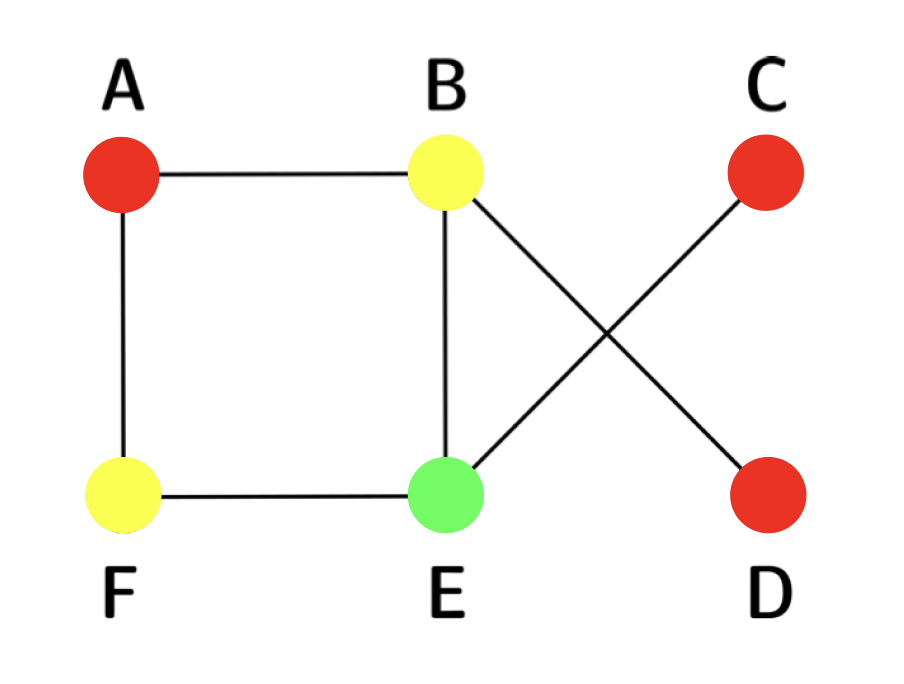
\includegraphics[scale=0.5]{coloring.png}
%      \caption{Coloring of the graph.}
% \end{figure}

% \begin{figure}[htb]
%     \qquad
%     \begin{minipage}{.4\textwidth}
%         \centering
%         {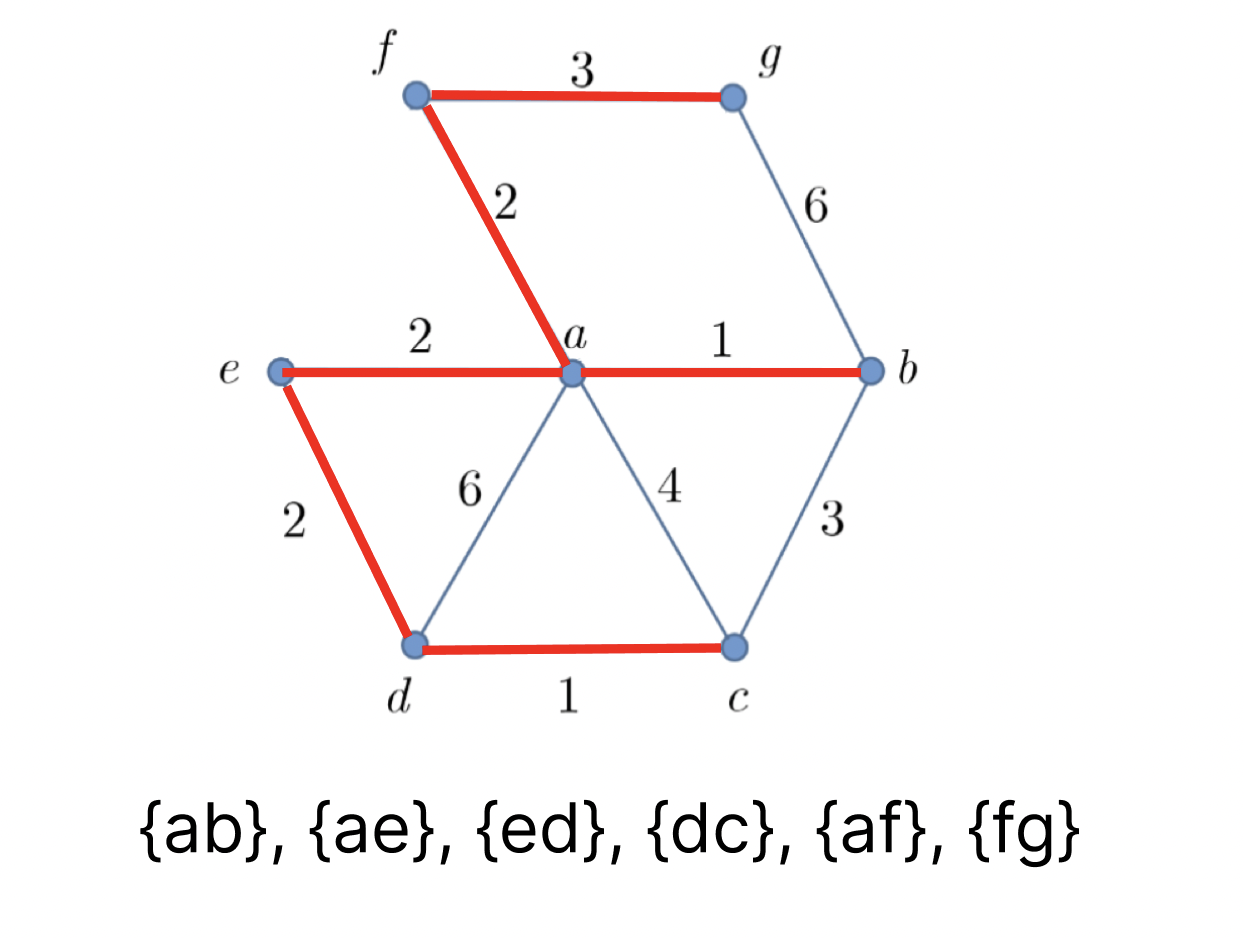
\includegraphics[scale=0.35]{prims.png}}
%         \qquad\qquad\emph{Prim's}\label{fig:1}
%     \end{minipage}    
%     \qquad
%     \begin{minipage}{.4\textwidth}
%         \centering
%         {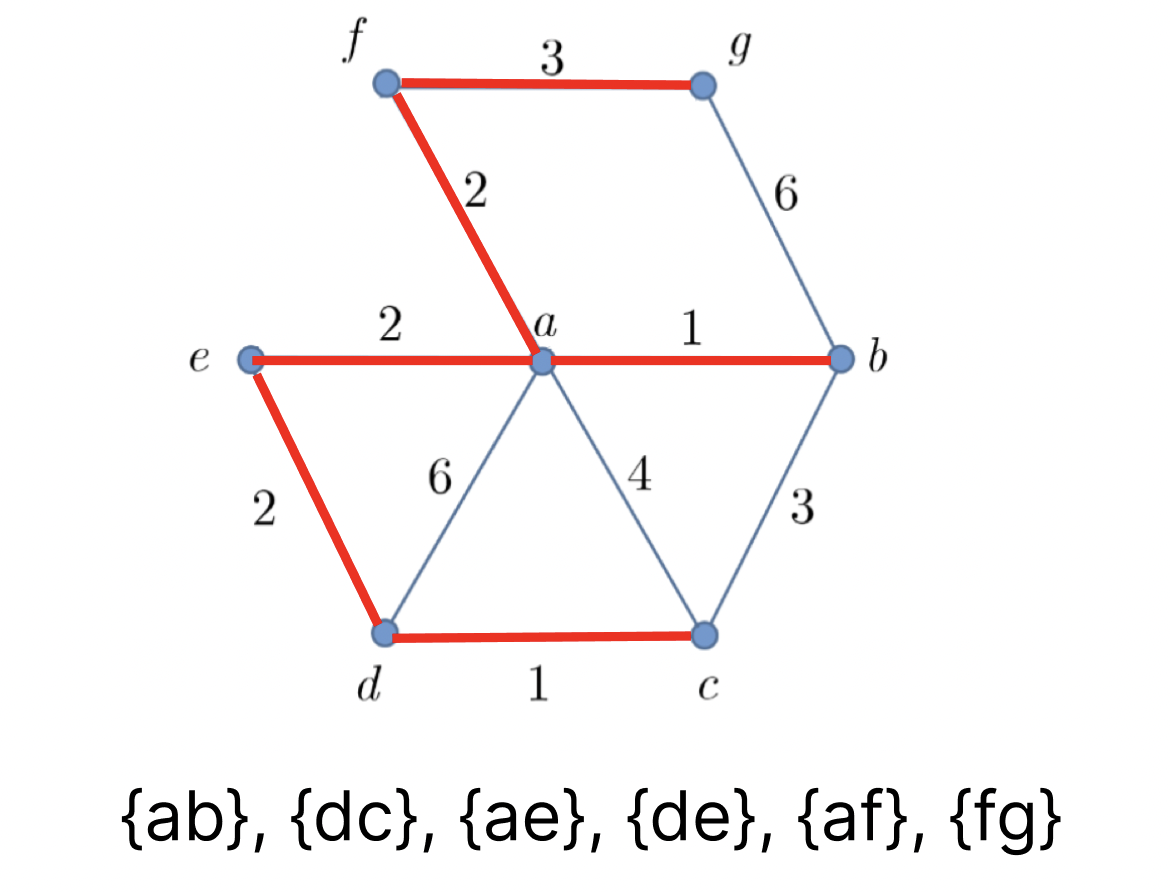
\includegraphics[scale=0.35]{kruskal.png}}
%         \qquad\qquad\emph{Kruskal's}\label{fig:2}
%     \end{minipage}        
% \end{figure} 

\newtheorem{thm}{Theorem}
\newtheorem{proposition}[thm]{Proposition}
\newtheorem{cor}[thm]{Corollary}

% title information
\title{Math 128A HW2}
\author{Neo Lee}
\date{09/13/2023}

\setstretch{1.15}
% main content
\begin{document} 

% placing title information; comment out if using fancyhdr
\maketitle 

\section*{Section 2.2}
\subsection*{Problem 1c}
Use algebraic manipulation to show that $$g_3(x)=\left(\frac{x+3}{x^2+2}\right)^{1/2}$$ has a fixed 
point at $p$ precisely when $f(p)=0$, where $f(x)=x^4+2x^2-x-3$.
\begin{proof}
    \begin{align*}
        f(p) = 0 & = p^4 + 2p^2 - p - 3 \\
        p^2(p^2 + 2) & = p + 3 \\
        p & = \left(\frac{p+3}{p^2+2}\right)^{1/2} = g(p).
    \end{align*}
\end{proof}

\subsection*{Problem 8}
Use a fixed-point iteration method to determine a solution accurate to within $10^{-2}$ for $x^3 
- x - 1 = 0$ on $[1,2]$. Use $p_0 = 1$.
\begin{proof}[Solution]
    Define $g(x):=(x+1)^{1/3}$. Then $g(x)=x$ when $x^3-x-1=0$. Indeed, $g(x) \in [1,2]$ for $x \in 
    [1,2]$ and $|g'(x)| < 1$ for $x\in[1,2]$. By the fixed-point theorem, we are sure that the 
    fixed-point iteration will converge to the solution. 
    
    \begin{figure}[htb!]
        \centering
        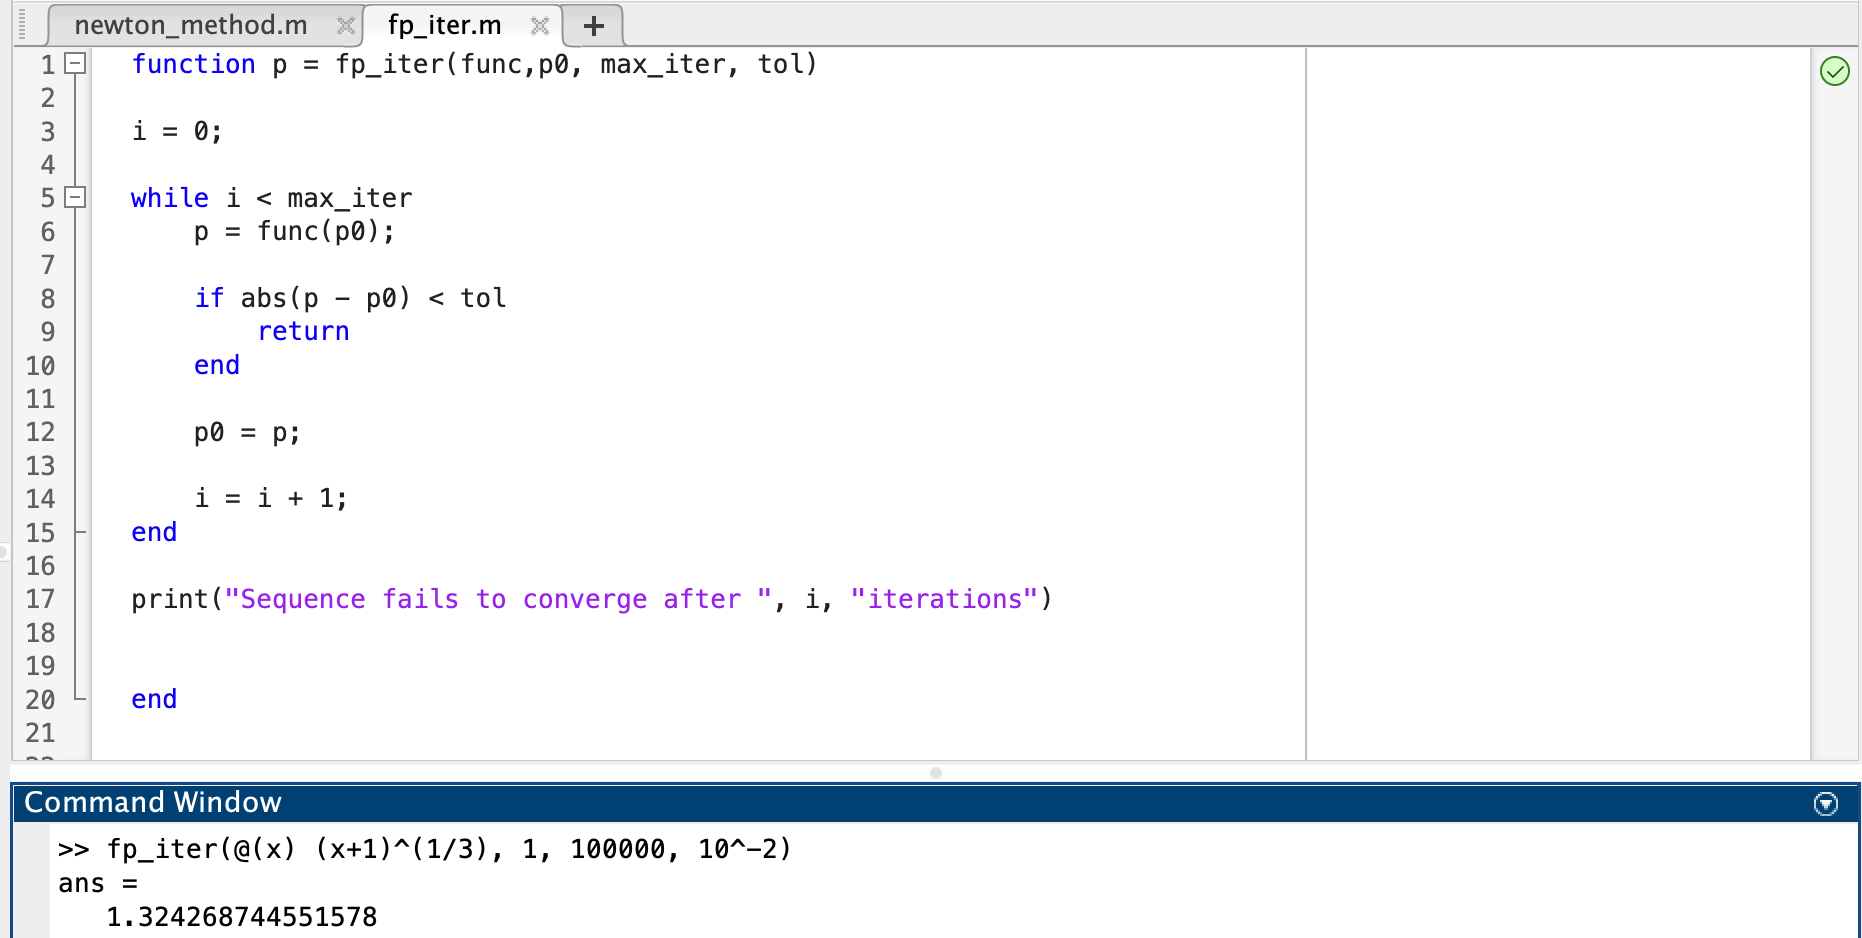
\includegraphics[scale=0.2]{2.2.8.png}
        \caption{$x = 1.3243$}
    \end{figure}
\end{proof}

\subsection*{Problem 19}
Let $g\in C^1[a,b]$ and $p$ be in $(a,b)$ with $g(p)=p$ and $|g'(p)|>1$. Show that there exists a 
$\delta > 0$ such that if $0<|p_0-p|<\delta$, then $|p_0-p|<|p_1-p|$. Thus, no matter how close the 
initial approximation $p_0$ is to $p$, the next iteration $p_1$ is farther away, so the fixed-point 
iteration does not converge if $p_0\neq p$.
\begin{proof}
    $|g'(p)>1|\Rightarrow |g'(p)| = 1 + \epsilon$ for some $\epsilon>0$. Since $g'$ is continuous, 
    there exists $\delta > 0$ such that for all $c\in(p-\delta,p+\delta)$, $|g'(c) - g'(p)| < 
    \epsilon\Rightarrow |g'(c)| > 1$. Now consider such $p_0\in(p-\delta, p+\delta)-\{p\}$,
    \begin{align*}
        |p_1-p| & = |g(p_0)-p| \\
        |p_1-p| & = |g'(\xi)(p_0 - p)| \qquad (\emph{for $\xi$ between }p_0, p) \\
        \frac{|p_1-p|}{|p_0-p|} & = |g'(\xi)| \\ 
        \frac{|p_1-p|}{|p_0-p|} & > 1. \qquad (\because \xi \in (p-\delta, p+\delta))
    \end{align*}
    
\end{proof}

\subsection*{Problem 20}
Let $A$ be a given positive constant and $g(x)=2x-Ax^2$.
\begin{enumerate}[label=\alph*.]
    \item Show that if fixed-point iteration converges to a nonzero limit, then the limit is 
    $p=1/A$, so the inverse of a number can be found by using only multiplications and subtractions.
    \begin{proof}[Solution]
        Let $g(p) = p = 2p-Ap^2$,
        \begin{align*}
            p & = 2p - Ap^2 \\
            Ap^2 - p & = 0 \\
            p(Ap-1) & = 0.
        \end{align*}
        Hence, $p=0$ or $Ap=1\Rightarrow \underline{p = 1/A}$.
    \end{proof}
    \item Find an interval about $1/A$ for which fixed-point iteration converges, provided $p_0$ is 
    in that interval.
    \begin{proof}[Solution]
        Define the interval $I = (\frac{1}{A}-|\frac{1}{2A}|, \frac{1}{A}+|\frac{1}{2A}|)$. Now 
        consider $c \in I$, $c$ can be written as  $\frac{1}{A} + \epsilon$ such that 
        $|\epsilon|<|\frac{1}{2A}|$. 
        \begin{align*}
            |g'(c)| & = |2 - 2Ac| \\
            & = |2-2A\left(\frac{1}{A}+\epsilon\right)| \\
            & = |2A\epsilon| \\
            & < |2A\cdot\frac{1}{2A}| \\
            & < 1.
        \end{align*}
        Now consider $g(c) - g(\frac{1}{A})$,
        \begin{align*}
            |g(c) - g(\frac{1}{A})| & = |g'(\xi)(c-\frac{1}{A})| \qquad (\xi \emph{ between }
            c, \frac{1}{A})\\
            |g(c) -\frac{1}{A}| & < 1 \cdot |c - \frac{1}{A}| \\
            |g(c) -\frac{1}{A}| & < |\frac{1}{2A}|.
        \end{align*}
        Hence, $g(c)\in I$.
        
        We have verified that for all $c\in I$, $g'(c)<1$ and $g(c)\in I$. Thus, by fixed point 
        theorem, the fixed-point iteration with $p_0 \in I$ will converge.
    \end{proof}
\end{enumerate}
\section*{Section 2.3}
\subsection*{Problem 6c}
Use Newton's method to find solutions accurate to within $10^{-5}$ for 
$$f(x) = 2xcos(2x) - (x-2)^2=0\qquad \emph{for } 2\le x\le 3 \emph{ and }3\le x\le 4.$$
\begin{proof}[Solution]
    \begin{align*}
        f'(x) & = -4xsin(2x) + 2cos(2x) - 2(x-2).
    \end{align*}
    
    Hence, for Newton's method, 
    \begin{align*}
        g(x) & = x - \frac{2xcos(2x)-(x-2)^2}{-4xsin(2x)+2cos(2x)-2(x-2)}.
    \end{align*}
    With the fixed-point iteration function coded in Section 2.2 problem 8, we have 
    \begin{figure}[htb]
        \qquad
        \begin{minipage}{.4\textwidth}
            \centering
            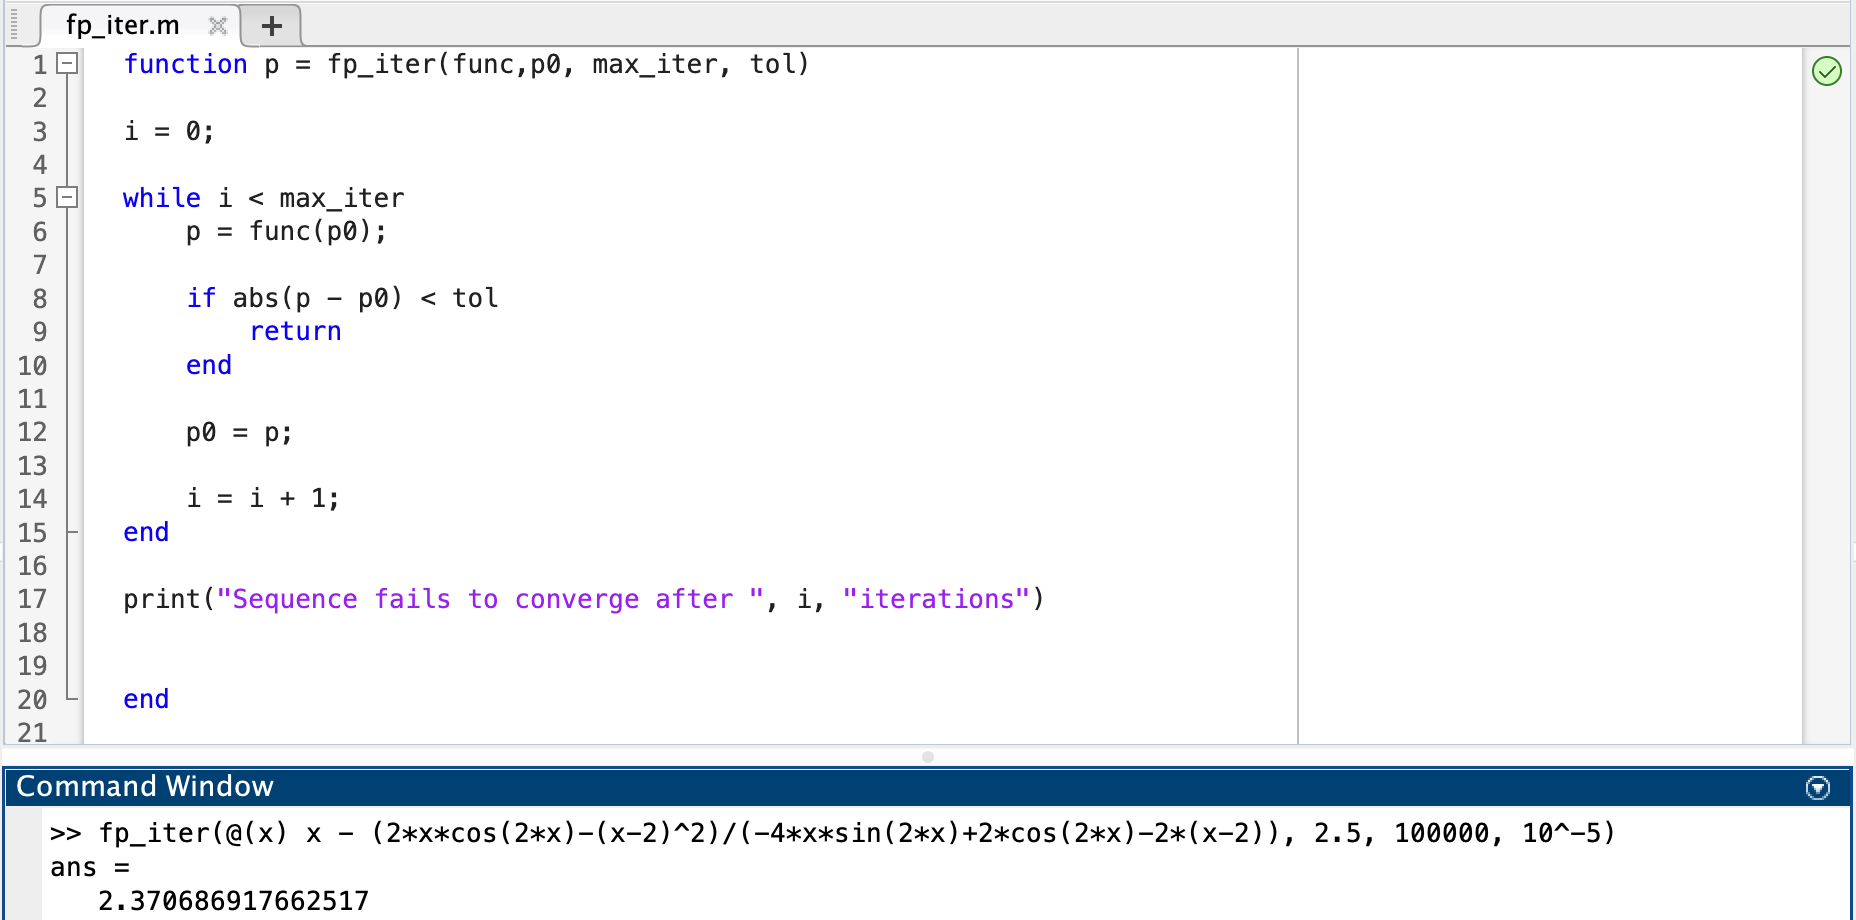
\includegraphics[scale=0.2]{2.3.6c1.png}
            \caption{$p_0 = 2.5 \in [2,3]$}
        \end{minipage}    
        \qquad
        \begin{minipage}{.4\textwidth}
            \centering
            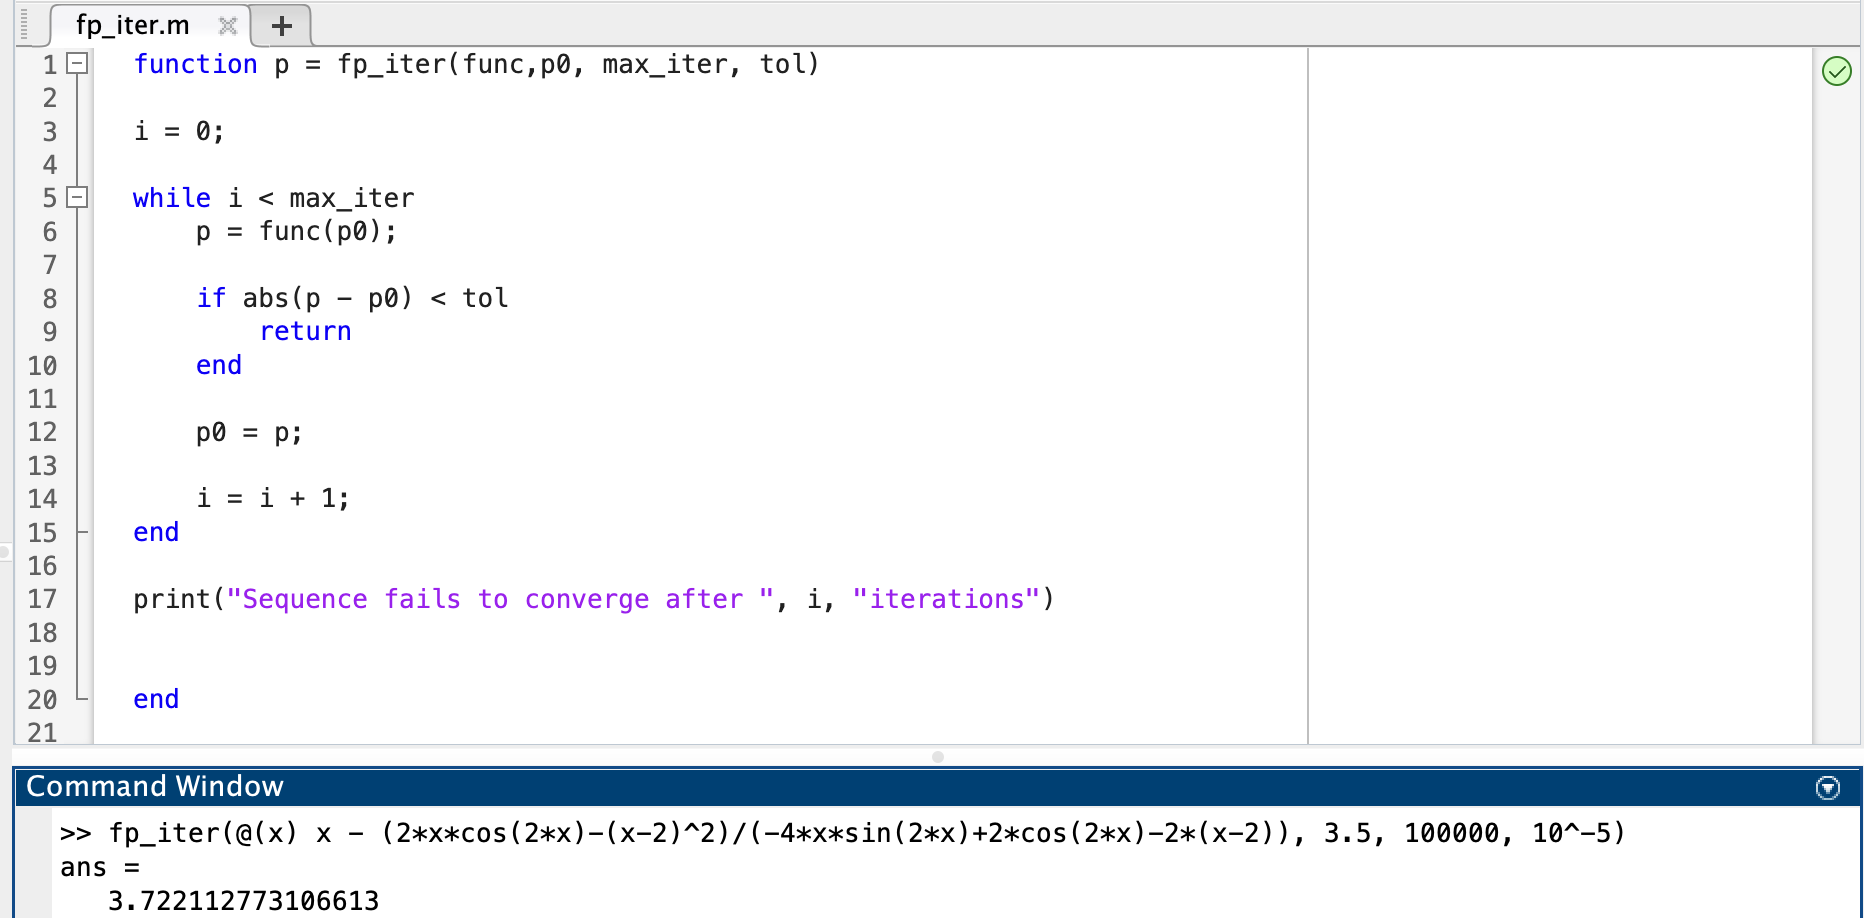
\includegraphics[scale=0.2]{2.3.6c2.png}
            \caption{$p_0 =3.5\in[3,4]$}
        \end{minipage}        
    \end{figure} 
\end{proof}

\newpage
\subsection*{Problem 8c}
Repeat 6c using the Secant method.
\begin{proof}[Solution]
    \begin{figure}[htb]
        \qquad
        \begin{minipage}{.4\textwidth}
            \centering
            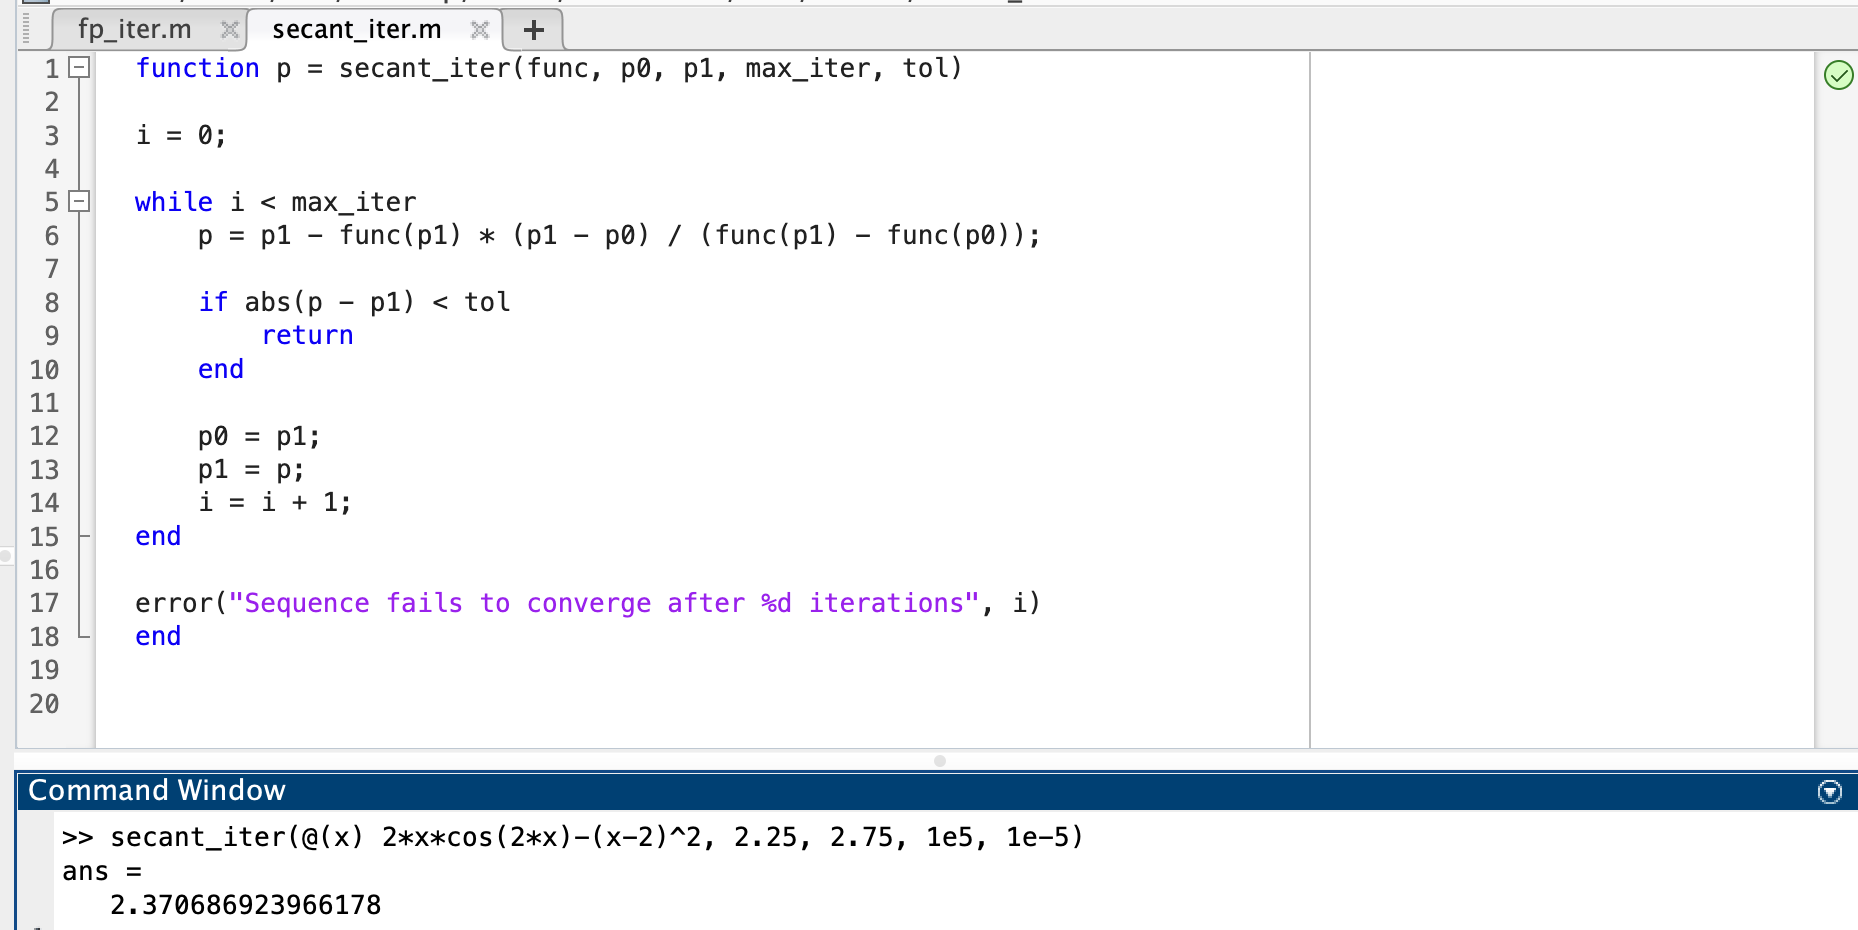
\includegraphics[scale=0.2]{2.3.8c1.png}
            \caption{$p_0 = 2.25, p_1 = 2.75$}
        \end{minipage}    
        \qquad
        \begin{minipage}{.4\textwidth}
            \centering
            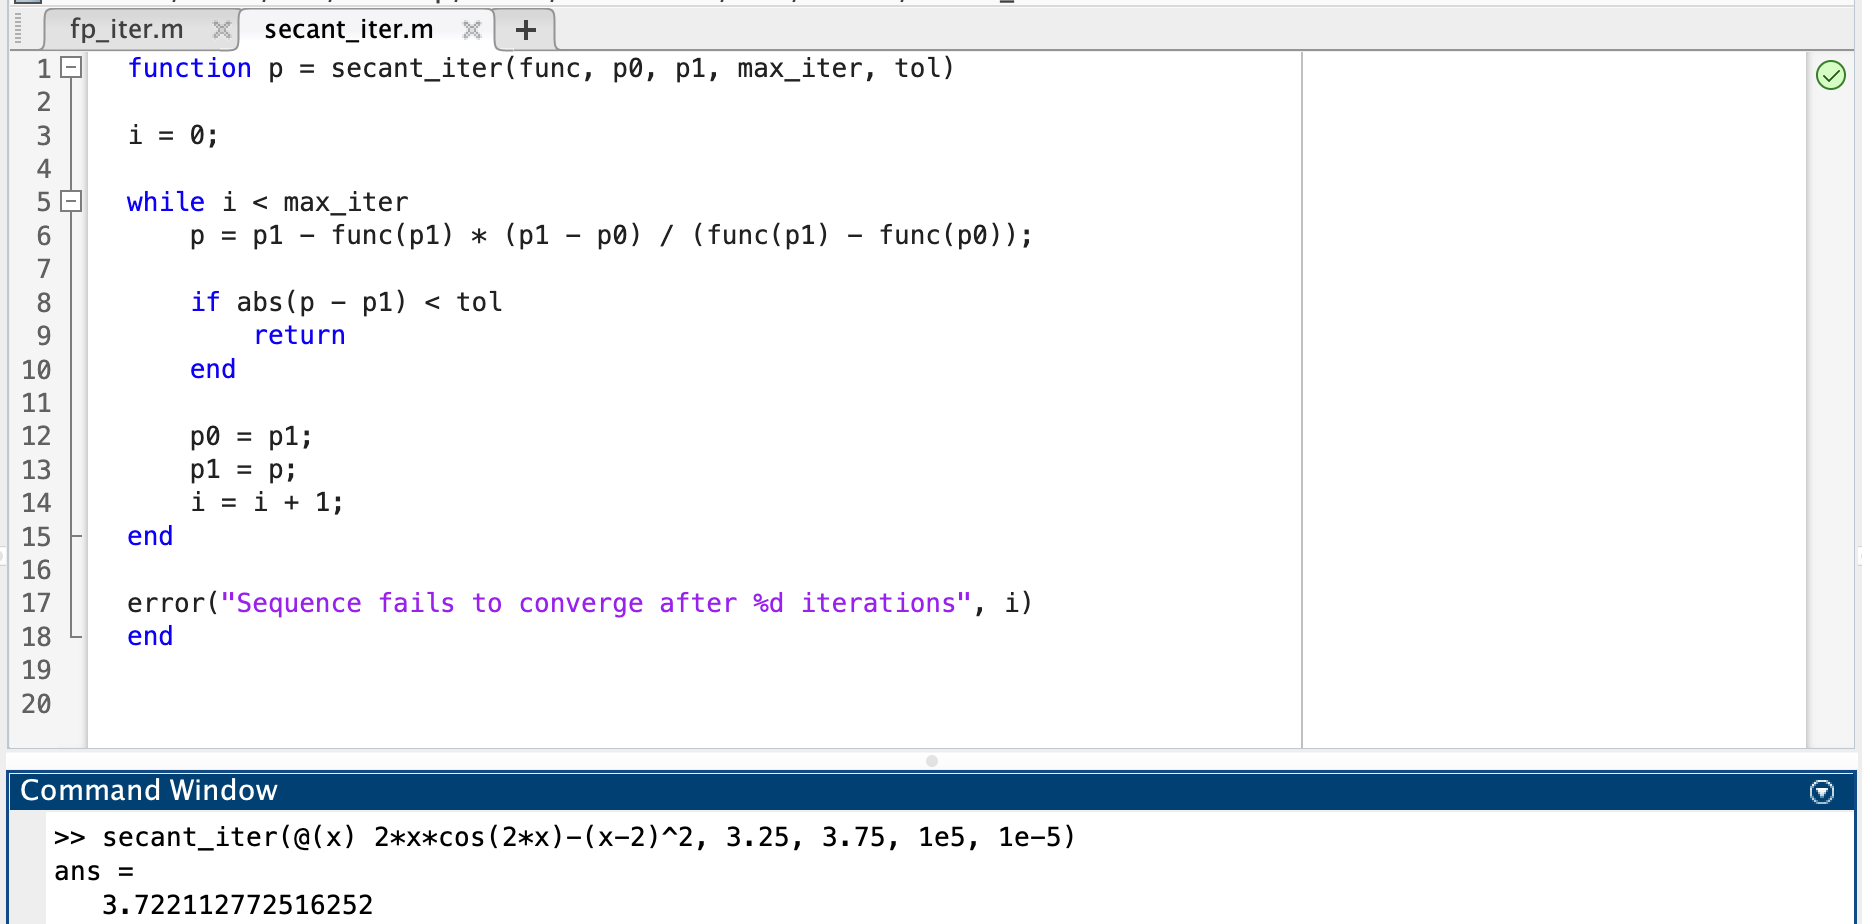
\includegraphics[scale=0.2]{2.3.8c2.png}
            \caption{$p_0 = 3.25, p_1 = 3.75$}
        \end{minipage}        
    \end{figure} 
\end{proof}

\subsection*{Problem 16}
Use Newton's method to approximate the solution of $f(x)=x^2-10cos(x)= 0$ to within $10^{-5}$ with 
\textbf{(a)}$p_0 = -100$ and \textbf{(d)}$p_0 = 25$.
\begin{proof}[Solution]
    \begin{align*}
        f'(x) & = 2x + 10sin(x) \\
        g(x) & = x - \frac{x^2-10cos(x)}{2x+10sin(x)}.
    \end{align*}
    \begin{figure}[htb]
        \qquad
        \begin{minipage}{.4\textwidth}
            \centering
            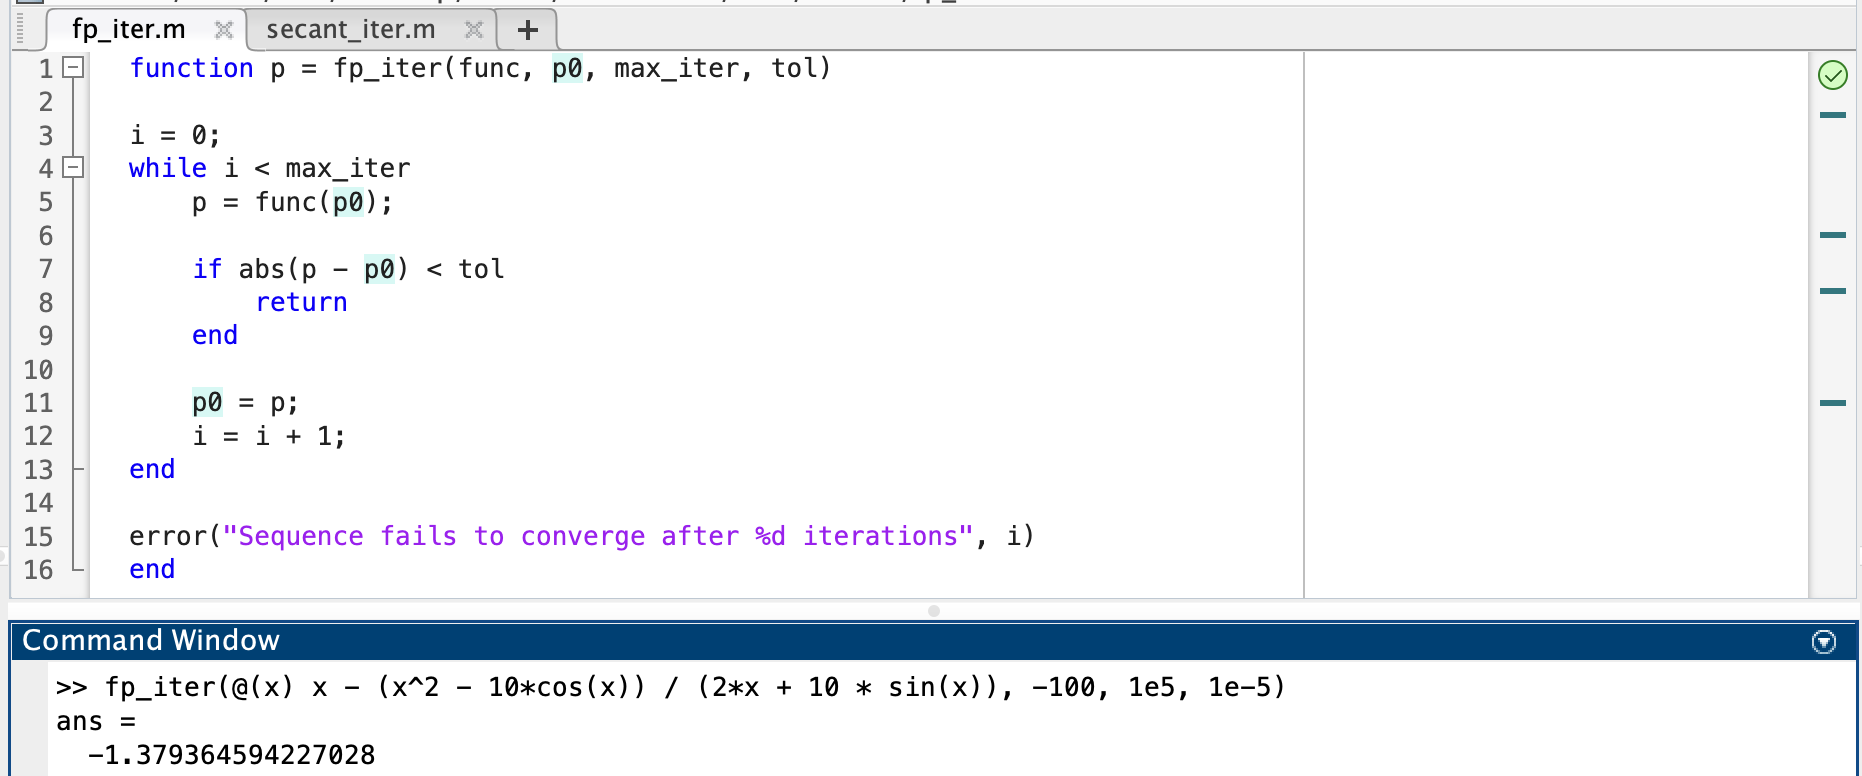
\includegraphics[scale=0.2]{2.3.16a.png}
            \caption{\textbf{(a)}$p_0 = -100$}
        \end{minipage}    
        \qquad
        \begin{minipage}{.4\textwidth}
            \centering
            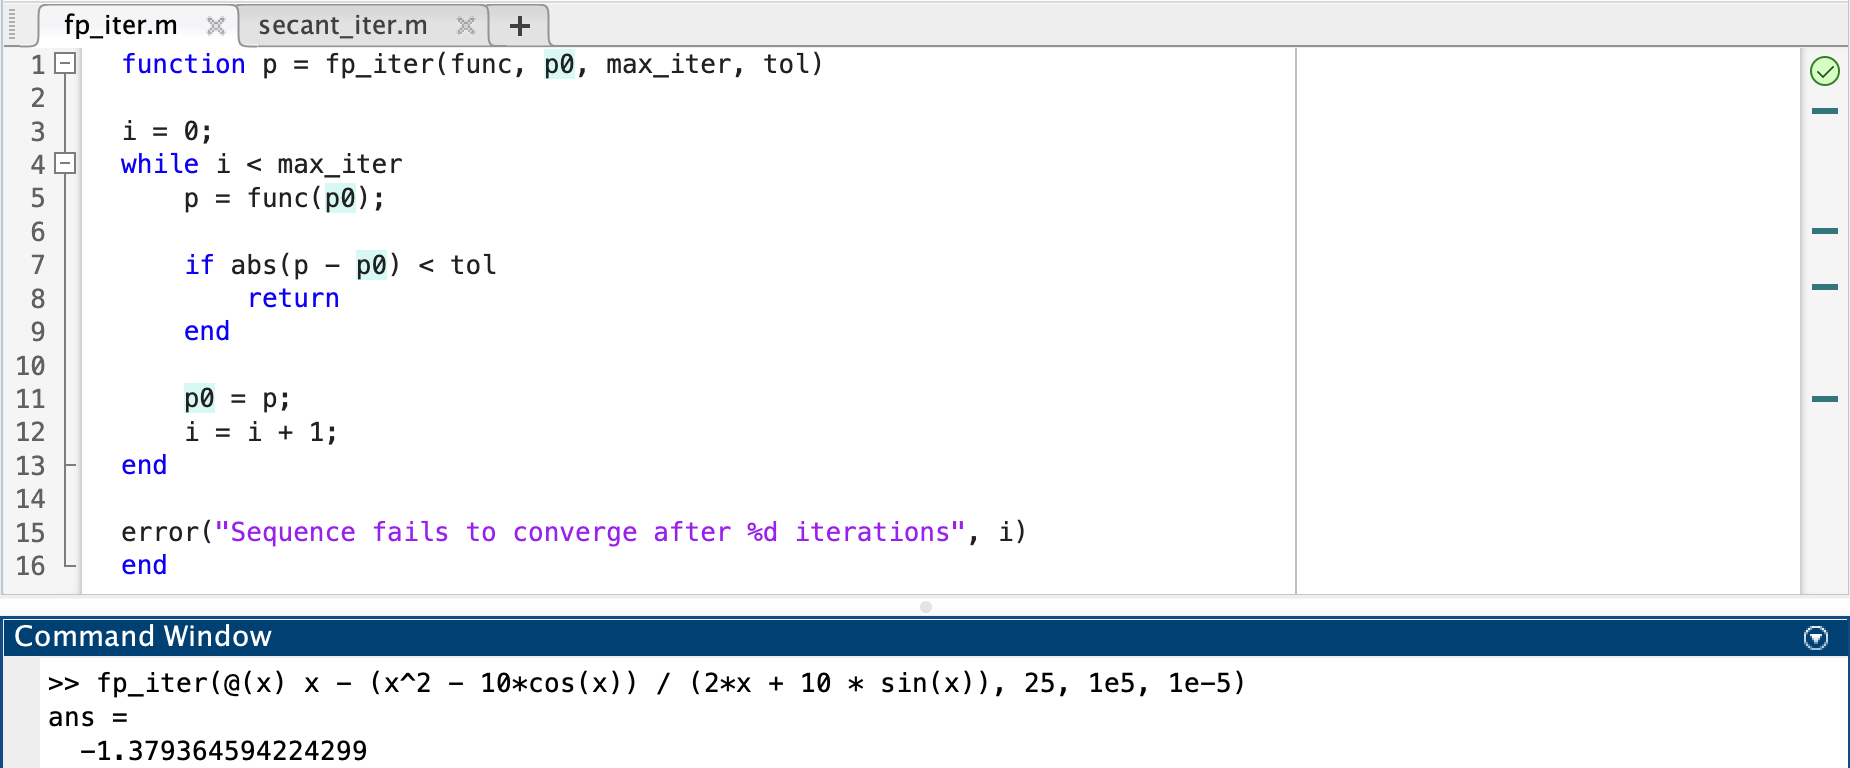
\includegraphics[scale=0.2]{2.3.16d.png}
            \caption{\textbf{(d)}$p_0 = 25$}
        \end{minipage}        
    \end{figure} 
\end{proof}

\newpage
\section*{Section 2.4}
\subsection*{Problem 2c}
Use Newton's method to find solutions accurate to within $10^{-5}$ to 
$$f(x)=sin(3x)+3e^{-2x}sin(x)-3e^{-x}sin(2x)-e^{-3x}=0 \qquad \emph{for }3\le x\le 4.$$
\begin{proof}[Solution]
    \begin{align*}
        f'(x) & = 3e^{-3x}\left(e^{3x}cos(3x)+e^{2x}sin(2x)-2e^{2x}cos(2x)-2e^xsin(x)+e^xcos(x)+1
        \right) \\
        g(x) & = x - \frac{sin(3x)+3e^{-2x}sin(x)-3e^{-x}sin(2x)-e^{-3x}}{3e^{-3x}\left(e^{3x}
        cos(3x)+e^{2x}sin(2x)-2e^{2x}cos(2x)-2e^xsin(x)+e^xcos(x)+1\right)}
    \end{align*}
    \begin{figure}[htb!]
        \centering
        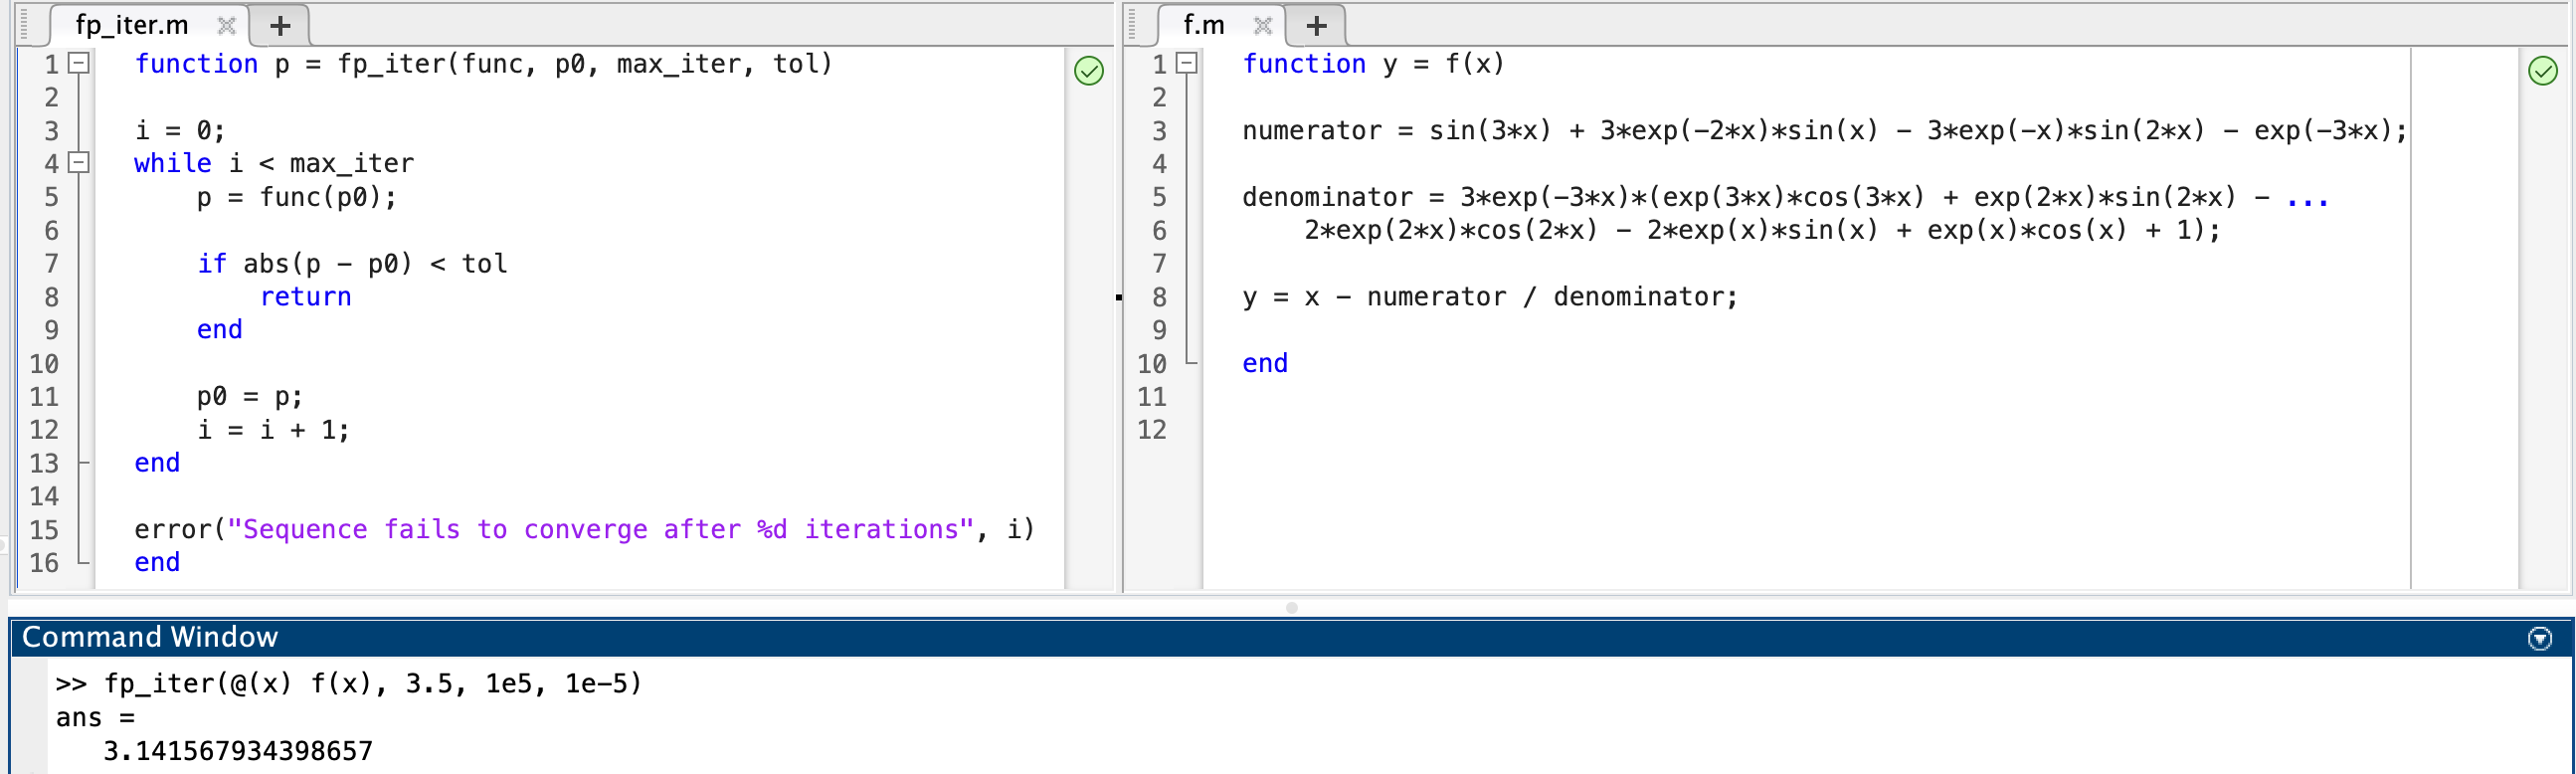
\includegraphics[scale=0.3]{2.4.2c.png}
        \caption{$x = 3.1415679$}
    \end{figure}
\end{proof}

\subsection*{Problem 8}
\begin{enumerate}[label=\alph*.]
    \item Show that the sequence $p_n = 10^{-2^n}$ converges quadratically to 0.
    \begin{proof}
        \begin{align*}
            10^{-2^{n+1}} & = 10^{-2^n \cdot 2} \\
            10^{-2^{n+1}} & = \left(10^{-2^n}\right)^2 \\
            |10^{-2^{n+1}}-0| & = |\left(10^{-2^n}\right)-0|^2 \\
            \frac{|10^{-2^{n+1}}-0|}{|\left(10^{-2^n}\right)-0|^2} & = 1 \\
            \lim_{n\rightarrow\infty}\frac{|p_{n+1}-0|}{|p_n-0|^2} & = 1.
        \end{align*}
    \end{proof}
    \item Show that the sequence $p_n = 10^{-n^k}$ does not converge to 0 quadratically, regardless 
    of the size of the exponent $k > 1$.
    \begin{proof}
        If the sequence converge quadratically, $\lim_{n\rightarrow\infty}\frac{|p_{n+1}|}{|p_n|^2} 
        = C$ for some positive constant C. Consider
        \begin{align*}
            \lim_{n\rightarrow\infty}\frac{|10^{-(n+1)^k}|}{|10^{-n^k}|^{^2}} & = 
            \lim_{n\rightarrow\infty}\frac{10^{-(n+1)^k}}{10^{-2n^k}} \\
            & = \lim_{n\rightarrow\infty}10^{-(n+1)^k+2n^k}.
        \end{align*}

        Now we evaluate 
        \begin{align*}
            \lim_{n\rightarrow\infty}-(n+1)^k+2n^k & = 
            \lim_{n\rightarrow\infty}\frac{-(n+1)^k+2n^k}{n^k}\cdot n^k \\
            & = \lim_{n\rightarrow\infty}\left(-\left(\frac{n+1}{n}\right)^k + 2\right)\cdot n^k \\
            & = \infty.
        \end{align*}

        Hence, the limit
        \begin{align*}
            \lim_{n\rightarrow\infty}\frac{|10^{-(n+1)^k}|}{|10^{-n^k}|^{^2}} & = \infty \neq C,
        \end{align*}
        and the sequence does not converge quadratically.
    \end{proof}
\end{enumerate}

\subsection*{Problem 9}
\begin{enumerate}[label=\alph*.]
    \item Construct a sequence that converges to 0 of order 3.
    \begin{proof}[Solution]
        Let $p_n = 10^{-3^n}$.
        \begin{align*}
            |10^{-3^{n+1}}| & = |10^{-3^n}|^{^3} \\
            \lim_{n\rightarrow\infty}\frac{|10^{-3^{n+1}|}}{|10^{-3^n}|^{^3}} & = 1.
        \end{align*}
    \end{proof}
    \item Suppose $\alpha > 1$. COnstruct a sequence that converges to 0 of order $\alpha$.
    \begin{proof}[Solution]
        Let $p_n = 10^{-\alpha^n}$.
        \begin{align*}
            |10^{-\alpha^{n+1}}| & = |10^{-\alpha^n}|^{^\alpha} \\
            \lim_{n\rightarrow\infty}\frac{|10^{-\alpha^{n+1}|}}{|10^{-\alpha^n}|^{^\alpha}} & = 1.
        \end{align*}
    \end{proof}
\end{enumerate}

\subsection*{Discussion question 4}
What is the difference between the rate of convergence and the order of convergence? Have they any 
relationship to each other? Could two sequences have the same rates of convergence but different 
orders of convergence, or vice versa?

\section*{Extra}
\subsection*{Question 1}
\subsection*{Question 2}

\end{document}
